\section{Analyse de différents modèles}

\subsection{Modèle de génération de texte}
Le modèle de génération de texte est un modèle de langage qui génère une séquence de mots. Ce modèle est basé sur un réseau de neurones de type LSTM (Long Short Term Memory).
\begin{figure}[H]
    \centering
    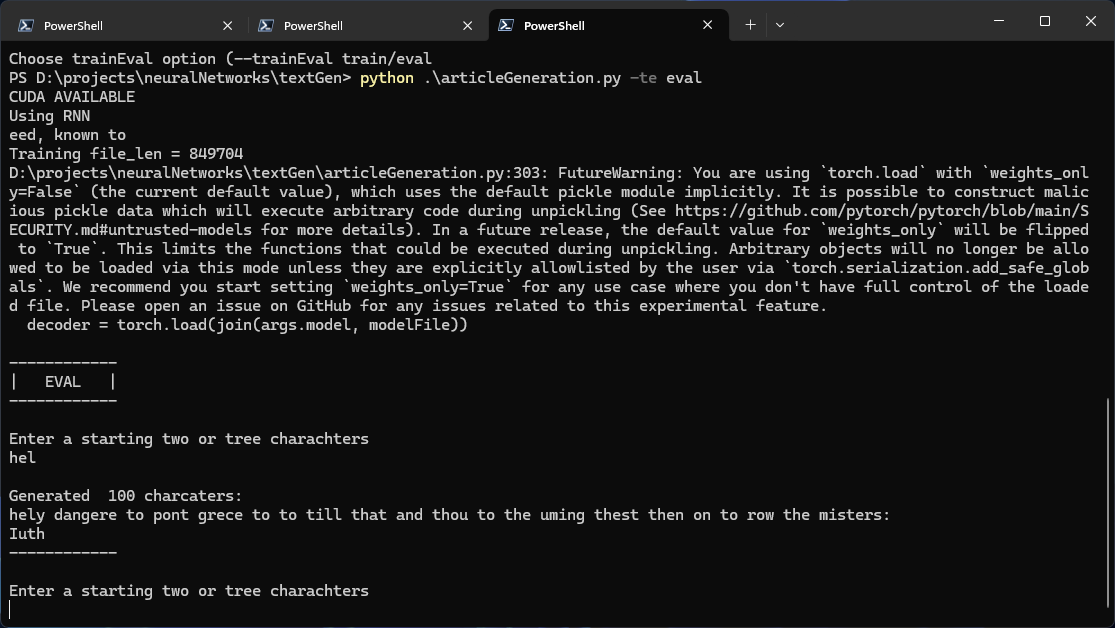
\includegraphics[width=.8\textwidth]{figures/shakespeare.png}
    \caption{Modèle de génération de texte}
    \label{fig:shakespeare}
\end{figure}

\subsection{Modèle de génération de noms russes}
Le modèle de génération de noms russes est un modèle de langage qui génère une séquence de caractères pour former un nom russe. Ce modèle est basé sur un réseau de neurones récurrents (RNN).
\begin{figure}[H]
    \centering
    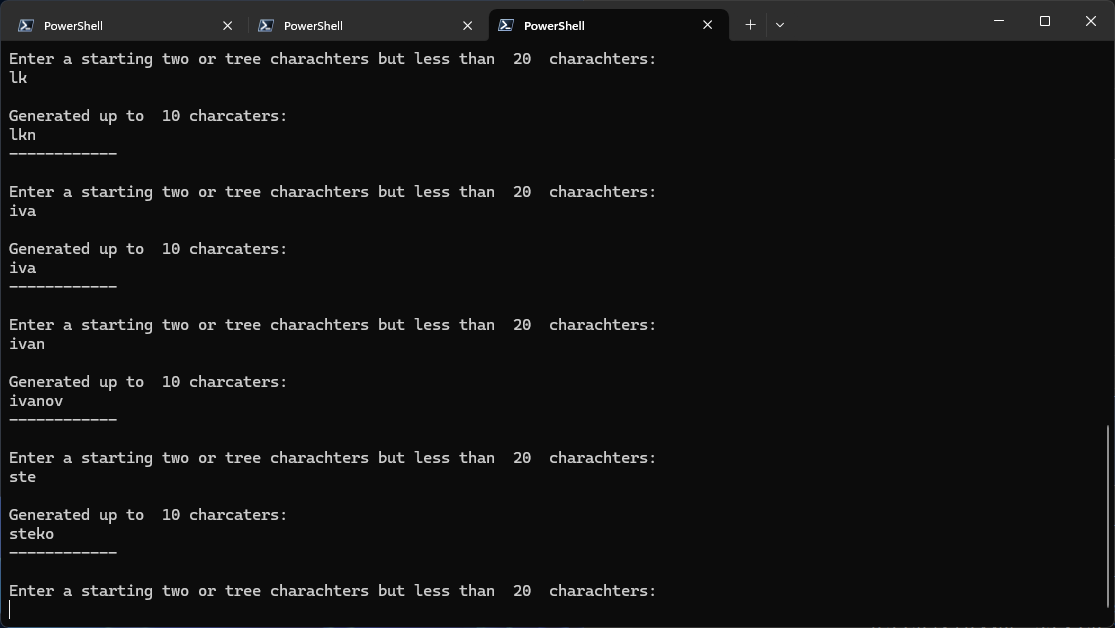
\includegraphics[width=.8\textwidth]{figures/russian.png}
    \caption{Modèle de génération de texte}
    \label{fig:russian}
\end{figure}

\subsubsection{Optimisation du modèle}
Afin d'optimiser le modèle de génération de noms russes, on a étudié i'impact de utisation des cellules GRU (Gates Recurrent Unit) \cite{pytorch_gru} au lieu de RNN, et on a comparé les résultats de chaque modèle avec les hyperparamètres suivants:
\begin{itemize}
    \item Nombre de couches: 2 $\rightarrow$ 8
    \item Nombre de couches cachées: 16 $\rightarrow$ 256
    \item Nombre d'époques: 10,000
    \item Taux d'apprentissage: 0.01 $\rightarrow$ 0.001 $\rightarrow$ 0.0001
\end{itemize}

\subsubsection{Taux d'apprentissage}
Au niveau des deux modèles, on remarque que les performances sont meulleures avec un taux d'apprentissage de 0.0001, où la précision atteint une valeur de 12\%.
\begin{figure}[H]
    \centering
    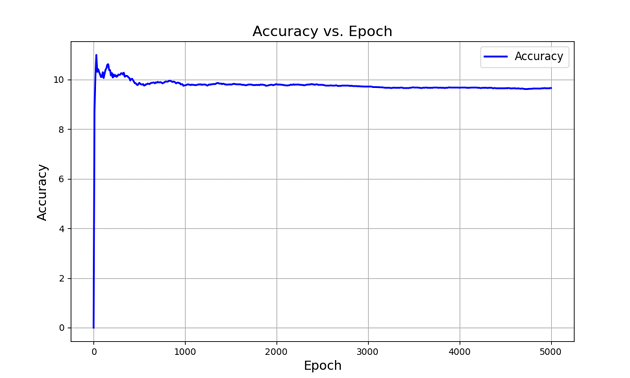
\includegraphics[width=.8\textwidth]{figures/0_01.png}
    \caption{Précision avec un taux d'apprentissage de 0.01}
    \label{fig:0_01}
\end{figure}

\begin{figure}[H]
    \centering
    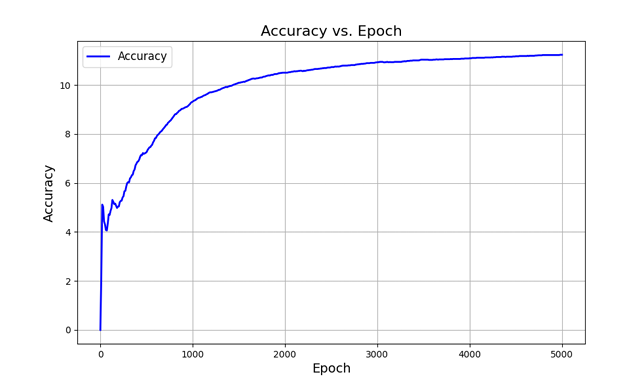
\includegraphics[width=.8\textwidth]{figures/0_0001.png}
    \caption{Précision avec un taux d'apprentissage de 0.0001}
    \label{fig:0_0001}
\end{figure}

\subsubsection{Taux de précision}
On remarque qu'avec les différents hyperparamètres, que les performances du modèle avec GRU sont un peu mieux que celles du modèle avec RNN (2\% en moyenne), mais le modèle avec RNN est plus rapide que celui avec GRU.
\begin{figure}[H]
    \centering
    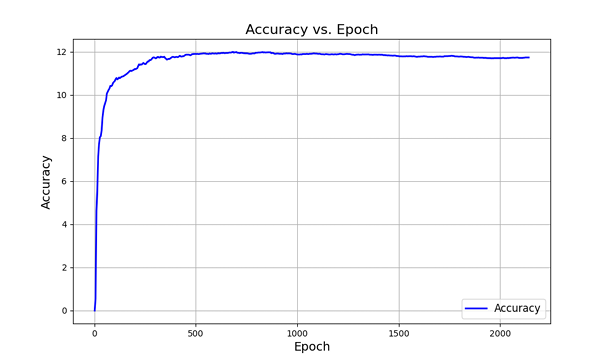
\includegraphics[width=.8\textwidth]{figures/gru.png}
    \caption{Précision du modèle avec GRU 12\%}
    \label{fig:gru}
\end{figure}
\begin{figure}[H]
    \centering
    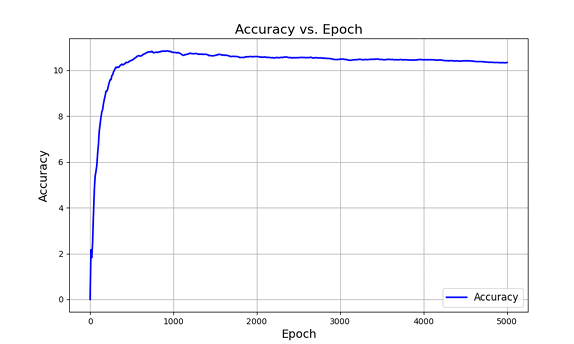
\includegraphics[width=.8\textwidth]{figures/rnn.png}
    \caption{Précision du modèle avec RNN 10\%}
    \label{fig:rnn}
\end{figure}

\subsubsection{Taux de pertes}
On remarque que au bout de 2,000 époques les pertes des deux modèles deviennent stable et ne changent pas beaucoup.
\begin{figure}[H]
    \centering
    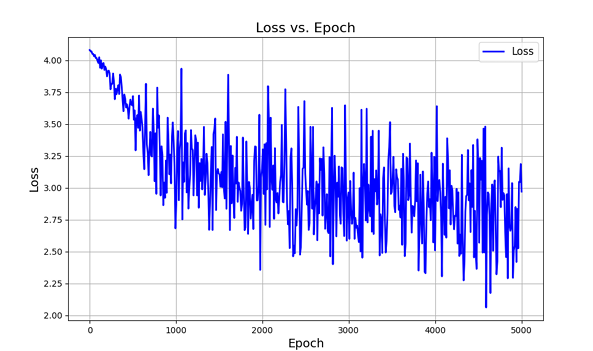
\includegraphics[width=.8\textwidth]{figures/loss_gru.png}
    \caption{Pertes du modèle avec GRU}
    \label{fig:loss_gru}
\end{figure}
\begin{figure}[H]
    \centering
    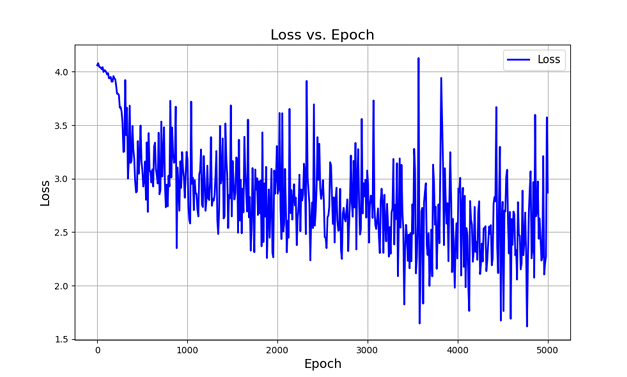
\includegraphics[width=.8\textwidth]{figures/loss_rnn.png}
    \caption{Pertes du modèle avec RNN}
    \label{fig:loss_rnn}
\end{figure}